\section{Self-Propelled Particles/Polar Active Fluids}

\subsection{Overview of Self-propelled particles}
Today we discuss self-propelled particles, also known as polar active fluids. Your next homework will be almost entirely devoted to this topic. This is a new type of active matter, compared to what you have seen thus far in the course. The first experiments on this topic can be found in \texttt{Pallaci et al.\ Science (2014)}, \texttt{Bricard et al.\ Nature (2013)}.

Those in the soft matter class will know that there is one equation that governs the dynamics of simple fluids, namely the Navier-Stokes equation. Those not in the course will learn a bit of simple and complex fluids on the fly.

To give a bit of a physical picture, we are imagining that we have a fluid channel, containing many colloids. In the absence of pressure gradient, we see Brownian motion, and in the presence of a pressure gradient, we will see colloid flow. Here we consider the possibility of ``active colloids''. One example - colloids can have assymmetry (``Janus Particles''), e.g. the two sides can be made up of different material. If we shine light on the particles, the different sides will heat up in different amounts, creating a gradient within the particle itself. It then acts like a rocket that launches fuel more in one direction than the other, triggering the motion.

Another example (which you will become intimately familiar with on the homework) - we can have colloidal rollers that can be polarized via an electric field. Then, by rotating the colloids, we can have the colloids individually flow. If we have a fluid of such colloids, they will want to roll and align with each other - thus without applying any pressure gradient (they are self-driven!), the colloids will spontaneously pick a direction and flow. We will want to derive and analyze the Navier-Stokes equations to describe such self-propelled fluids. On your homework, you will first see how you can get a single particle to self-propel. Then, you will study the linear spectrum/excitations of such a medium. Finally, you will look at non-linear excitations, wherein the colloidal rollers move with a band structure.

You might imagine that there are interesting microfluid experiments that could be done with such exotic fluids. You can engineer lattices to contain such active fluids, and study what the properties of such a lattice are. In a Lieb lattice, such rollers rotate with alternating directions (chirality)! 

\begin{center}
    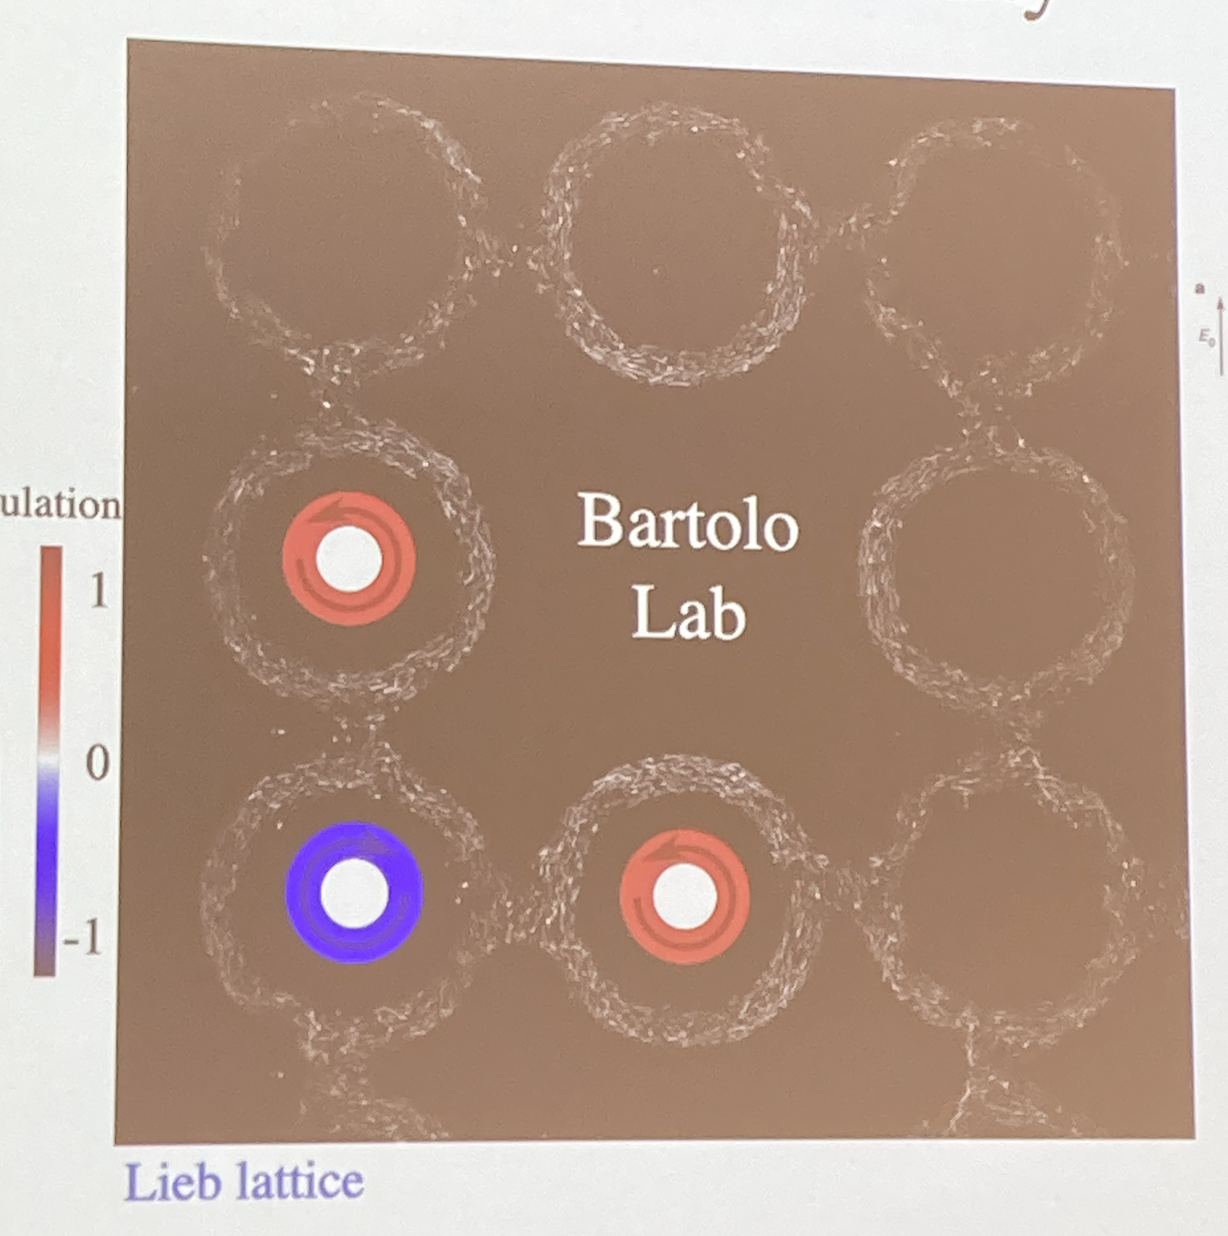
\includegraphics[scale=0.35]{Lectures/Images/lec8-circulation.png}
\end{center}

You can then also study what the sound modes of a channel made of such a fluid would look like - this your task in the homework, to look at density modulations on top of a nonzero velocity field. The sound waves will have a strange structure - density waves that go along with the flow and against the flow will have very different behaviours. You can even put this problem on steroids (\texttt{Souslov, van Zuiden, Bartolo, Vitelli.\ Nature (2017)}), and study such waves in not just one channel but in a 2D lattice - it turns out you can make a topological insulator out of such a lattice! Looking at the band structure, the bulk is gapped. But at the edge, you can have a density wave/excitations, and it is a directed excitation; it travels in a specific direction. In fact such excitations are topologically robust, in that they can flow around obstructions.

\begin{center}
    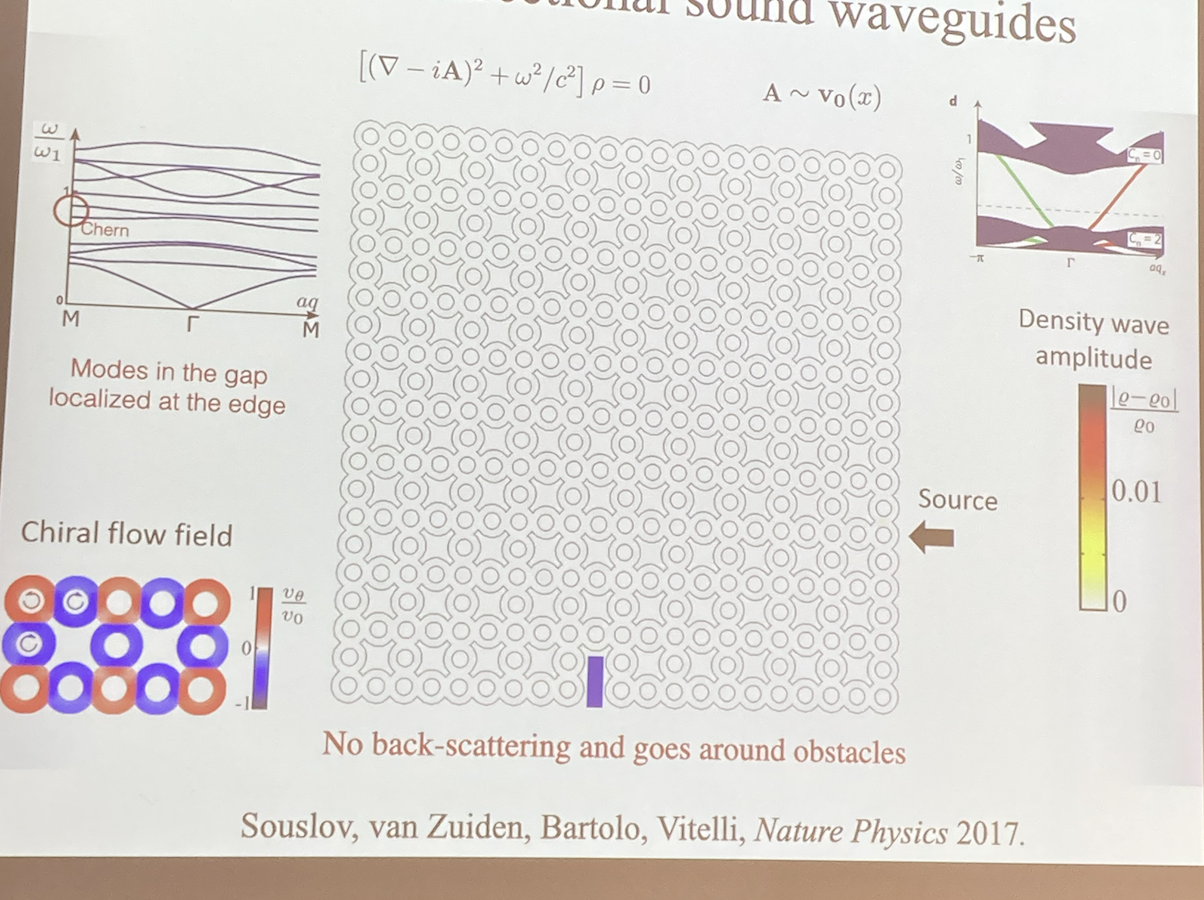
\includegraphics[scale=0.35]{Lectures/Images/lec8-lattice.png}
\end{center}

\subsection{Vicsek Model}
We will study the microscopic model that started this field - the Vicsek model of flying spins. The hydrodynamics of this model shows flocking\footnote{Everyone calls this flocking, but no one asked how the birds feel about it...} behaviour and phase transitions, and will be a useful model for understanding the more contemporary models of active matter that have come after it.

We consider a collection interacting bodies, and consider a mechanism in which the bodies move and align align. Consider the picture below:

\begin{center}
    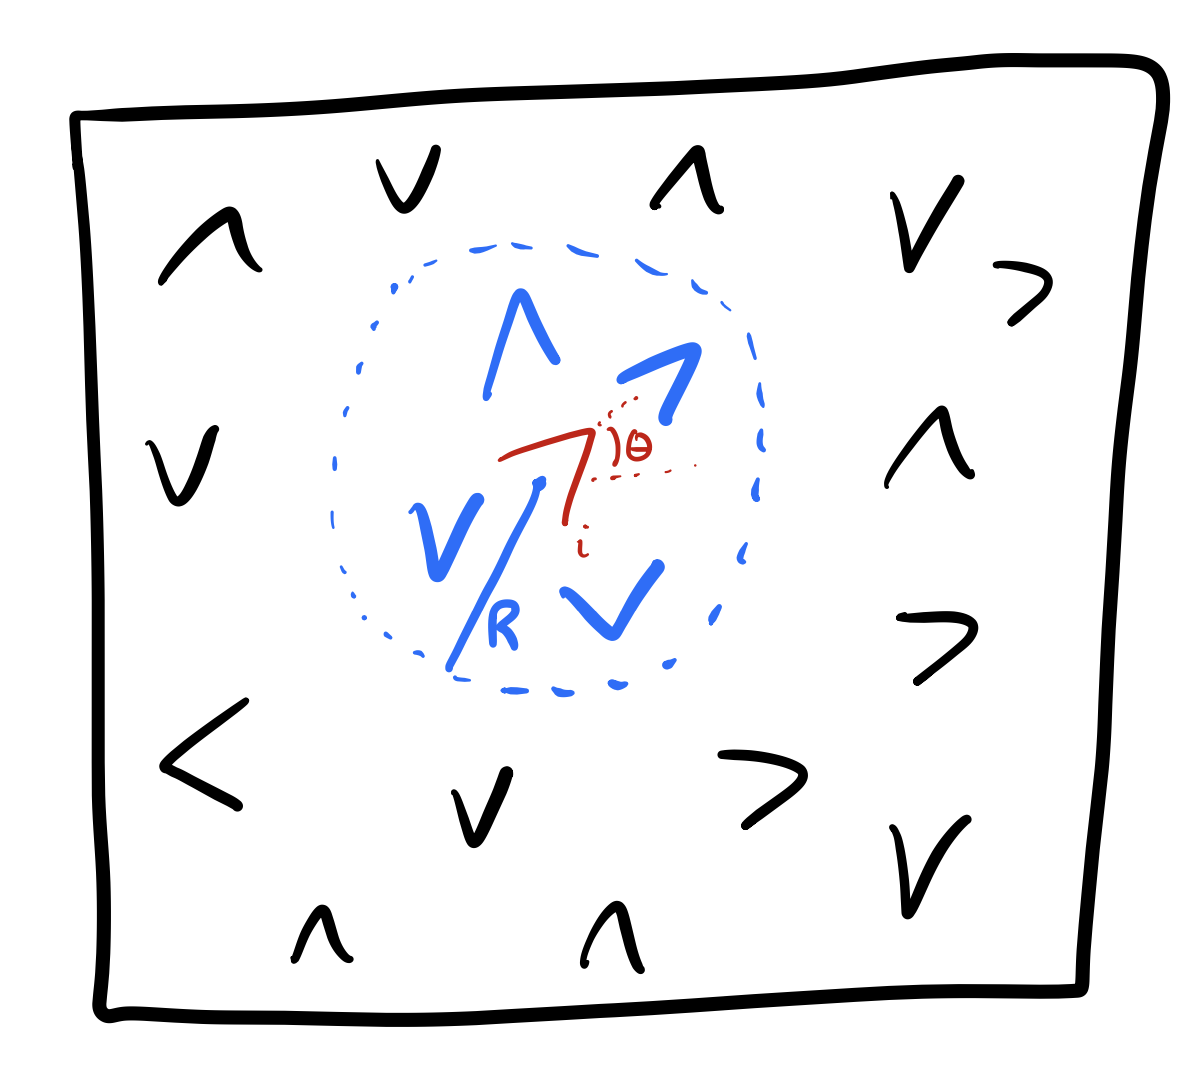
\includegraphics[scale=0.35]{Lectures/Images/lec8-Vicsek.png}
\end{center}

The update rule for the position of the $i$th body is:
\begin{equation}
    \v{r}_i(t + \Delta t) = \v{r}_i(t) + v_0\Delta t\m{\cos(\theta_i(t)) \\ \sin(\theta_i(t))}
\end{equation}
i.e. it takes one step in the direction it is facing. The update rule for the angle/direction of the $i$th body is:
\begin{equation}
    \theta_i(t + \Delta t) = \avg{\theta(t)}_{R, i} + \eta_i(t)
\end{equation}
where the first term corresponds to taking the average over the interaction range $R$ of other bodies. $\eta_i(t)$ is a noise term. In the Vicsek model, we can assume that the noise has zero mean:
\begin{equation}
    \avg{\eta_i(t)} = 0
\end{equation}
and has correlation (time average):
\begin{equation}
    \overline{\eta_i(t)\eta_j(t')} = 2\gamma\delta_{ij}\delta_{tt'}
\end{equation}
i.e. the noise is uncorrelated across space and time. The noise is local and Markovian (no memory), sometimes this is also called white noise.

Why is it called flying spins? The alignment of the direction of the bodies is like magnetic/spins which want to align with their neighbours, plus thermal fluctuations. The non-equilibrium dynamics comes from the fact that the spins can move! If the spins were fixed, you can just take the second equation and write down an equlibrium field theory (namely the XY model). But by coupling it into a self-propulsion rule, the model is non-equilibrium! 2D is interesting because the Mermin-Wagner theorem prevents the long-range ordering of the entire system in equilibrium settings.

Vicsek then studied this model just by numerically simulating it (this would be a good thing for you to also simulate as an exercise!) - see \texttt{Vicsek et al.\ PRL (1995)}

For high noise, we are in the disordered phase where the various spins fly in seemingly random directions. In the low noise, we are in the ordered/flocking phase where all spins move in the same direction. In this phase, we have a nonzero net velocity vector.

\begin{center}
    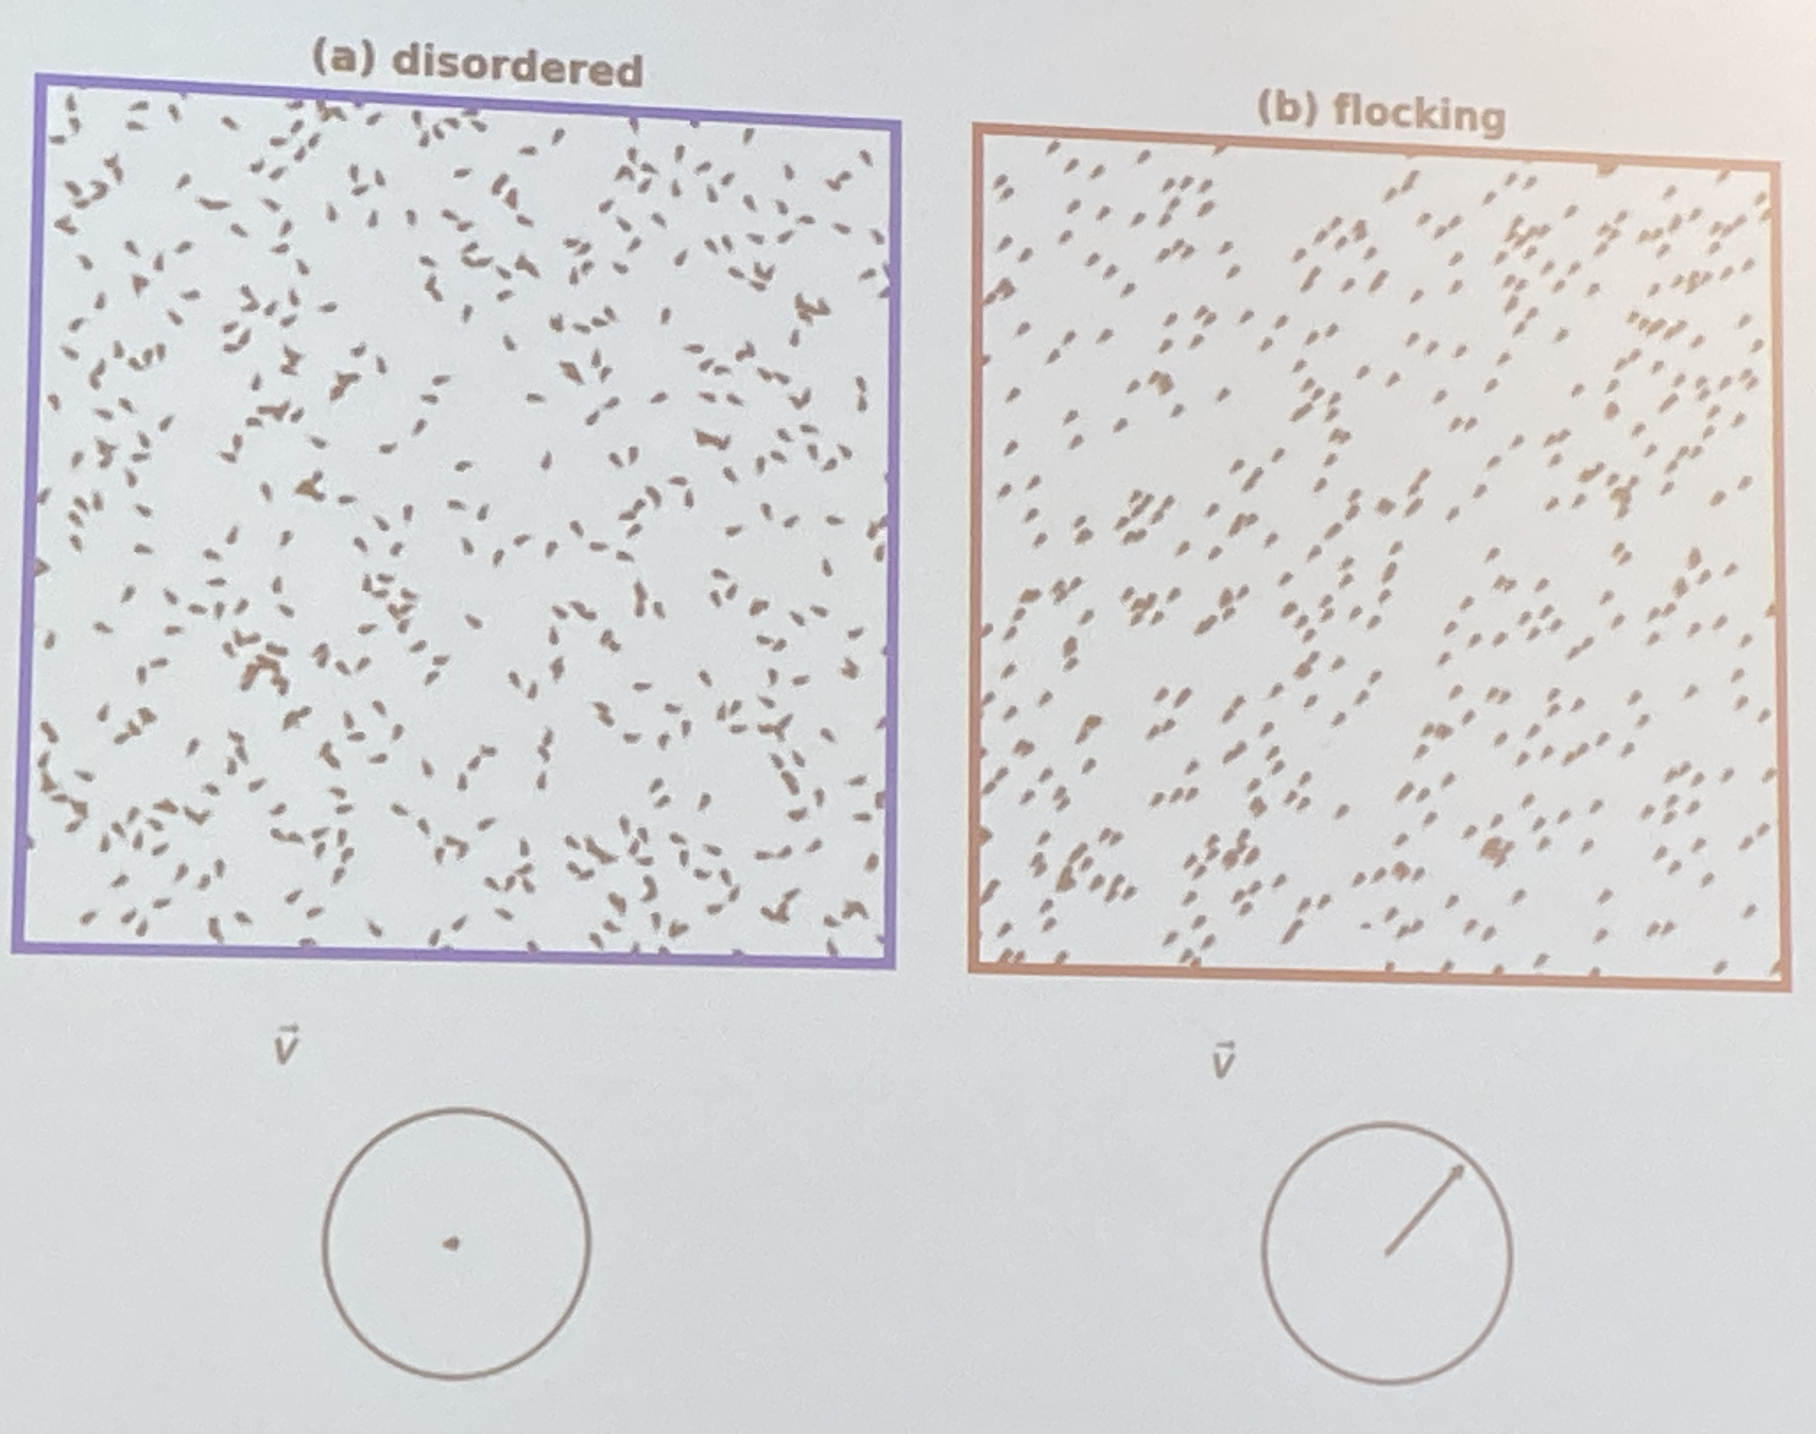
\includegraphics[scale=0.35]{Lectures/Images/lec8-flocking.png}
\end{center}

If we wanted to promote this to a continuum description, we could write down the energy:
\begin{equation}
    E = J\int d^2\v{x}(\nabla \theta)^2
\end{equation}
If $\frac{J}{k_B T} \ll 1$, thermal fluctuations are strong and we have disorder. For $\frac{J}{k_B T} \gg 1$, it is less clear. In equilibrium settings, in 2D Mermin-Wagner forbids long-range order. But here we have the coupling of the XY spin model to the self-propulsion model, which allows for the restoration of long-range order!

\subsection{Toner-Tu Model}
See \texttt{Toner, Tu.\ PRL (1995)} for the original paper.

Now, we will do some phenomenology; we will use the known symmetries of the theory and write down a macroscopic theory. As long as we are smart about it, we will get sensible results. However, we will not get the correct parameter dependencies of the macroscopic model on the microscopic parameters. Let us proceed. What we notice is that depending on the ratio $\frac{J}{\eta}$, we have either disordered or ordered behaviour. If you have taken a course on statistical field theory, you would have seen Landau theories of phase transitions, where we can write down an energy landscale that depends on a continuum spin parameter:
\begin{equation}
    E = J\int d^2\v{x}\left[(\nabla S)^2 + \alpha S^2 + \beta S^4\right]
\end{equation}
In the limit where $S$ is uniform, the gradient drops out. Then, depending on the $\alpha$ we either have a single minimum at $S = 0$ or degenerate minima at $S = \pm S_0$ (in 2D, we promote the two degenerate minima to a ring of minima, imagine a Sombrero). We can write $\alpha = c(T - T_c) = -c\e$, wherein for $T > T_c$ we have a single mimima and $T < T_c$ we have the degenerate minima. Usually in Landau theory we think about the system being in the energy minimizing configuration. We can also think about the dynamics at which the system comes to an energy minimizing configuration:
\begin{equation}
    \p_t S = -\frac{\delta V(S)}{\delta S}
\end{equation}

In our case, instead of a continuum spin/magnetization we instead have a velocity field. We have the potential:
\begin{equation}
    V(\v{v}) = -\alpha \v{v}^2 + \beta \v{v}^4
\end{equation}
Which taking the variation we get:
\begin{equation}\label{eq:TTbifurcationterms}
    \rho \p_t \v{v} = \alpha \v{v} - \beta \abs{\v{v}}^2 \v{v}
\end{equation}
This describes the bifurcation, but not the fluid aspects of the system. The pictures look like:

\begin{center}
    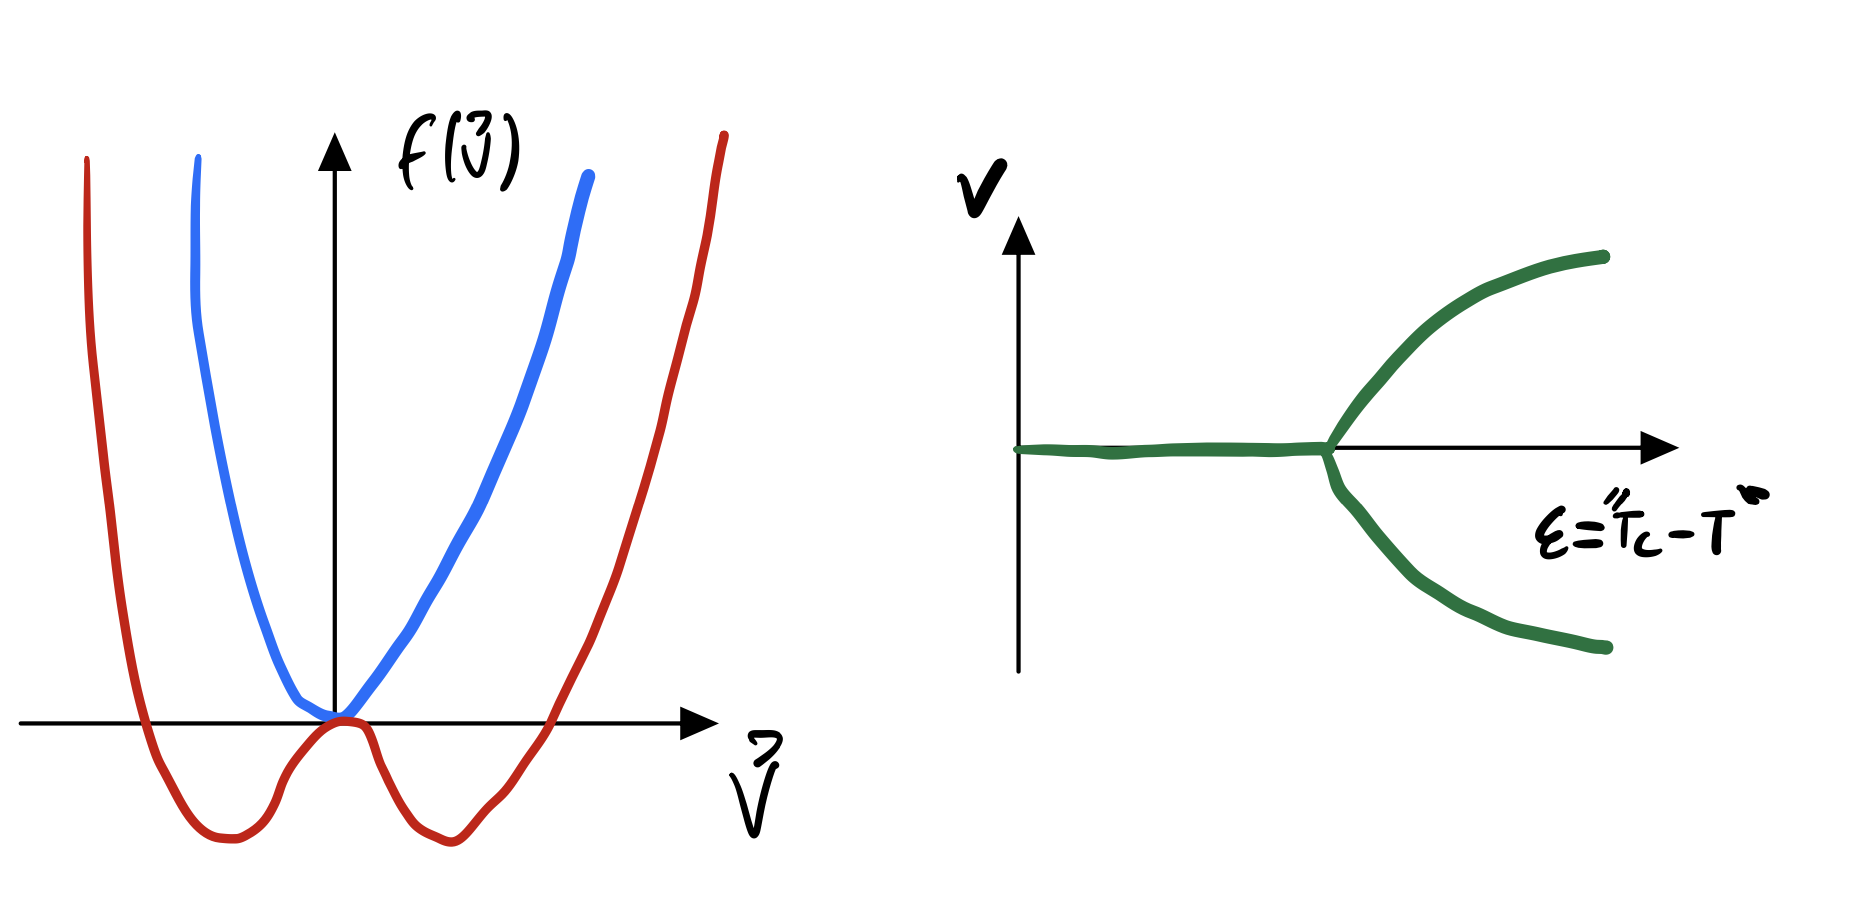
\includegraphics[scale=0.35]{Lectures/Images/lec8-bifurcation.png}
\end{center}

Where for $\e > 0$ we have pitchfork bifurcation. Much like in the magnet case, as a function of noise (temperature) we have a phase transition as detectable in the velocity (magnetization).

To account for the fluid aspects of the system, we think back to Navier-Stokes. One equation is the continuity/density conservation equation:
\begin{equation}
    \p_t \rho + \nabla \cdot (\rho\v{v}) = 0
\end{equation}
and from the other equation, we get insight on how to modify Eq. \eqref{eq:TTbifurcationterms} - we add pressure and viscosity terms on the RHS, as well as the convective term on the LHS:
\begin{equation}
    \boxed{\rho\left[\p_t \v{v} + \lambda_1(\v{v} \cdot \nabla)\v{v}\right] = -\nabla P + \eta \nabla^2\v{v} + \alpha \v{v} - \beta\abs{\v{v}}^2\v{v}}
\end{equation}
Note the one deviation from Navier-Stokes; there the invariance under boosts enforced $\lambda_1 = 1$, but we lose that here now that there is a preferred velocity. The above is the so-called Toner-Tu model. Minimally, it is as if we ``glue together'' pitchfork bifurcation with Navier-Stokes.